\newpage
\section{Development Process}

This chapter will provide a detailed description the methodology, and how we used it. It will describe some of our sprints and the project process as an entirety. There will also be a graphical view of the sprints showing the progress, and explanations over changes in the project scope.


\subsection{Scrum}

%% basic info about scrum?
%scrum is and agile development model, which allows for an iterative development cycle with a focus on completing work in 2-4 week long sprints. (add source here). 
%% compare canban and scrum, as they are both agile

For this project we chose to use scrum, as it allows us to quickly adapt to changing requirements. Due to the freedom given in this task this methology seamed to be the best fit. Scrum also allows us to quickly iterate on features, in order to get feedback from Lokførerskolen. 
The agile nature of scrum allows us to plan and divide the work into issues during the project. As such, we only divided work and created issues for the milestone currently in progress. This allows us to focus on the milestone at hand, without worrying about planning what to do in a future milestone where requirements or tasks might change.

In addition we have experience using scrum, as we used scrum in a previous course. Therefore we have experience with the workflows and structure used in Scrum. 

% HOW WE USED SCRUM
In the start of the project we used scrum strictly as described in the project plan[Link], where we had daily scrum meetings every day and sprint planning meetings in the beginning of each sprint. After the fourth sprint we decided to stop with the daily scrum meetings, the decision was mostly based on the value we got from the meetings. In the project planning phase we thought that the group was going to work individually and that it could be hard for everyone to keep an overview of the project. 

%% talk about jira, which we use to track sprints
In this project we used Jira for Scrum related work, such as creating sprints and to track milestones, stories, and issues. 

Jira also gives reports and graphs on the rate of work and issues created and finished during the project. 



another agile development model which we considered is canban, which is based on a board of tasks, where only a certain amount of tasks can be in progress at the same time. (add source here) 

%% code convention? process of learning unreal? 

\subsection{Methodology}

%% how we worked and our routines?

The group agreed on having workdays be from Monday to Friday, with standard work hours from 09.00 to 15.00. During this time 

workdays are mon-fri
workdays from 09.00 to 15.00 
time and days can be deviated from as needed, just notify the group

how we worked together
work from home, sit in voice chat room during workday
work is mostly solo on features, but we cooperate when merging features, working on common functionality, fixing problems or teaching each other stuff.
time tracking on jira using clockify addon, provides time tracking available for each issue


small daily meeting at the start of the day, stopped doing after a while
started with 1 week sprint length, switched to 2 weeks after main goal mvp was done
sprint meeting at start of week, group discusses progress and what issues to include in the next sprint

supervisor meetings
client meetings
retrospective meetings \& ... meetings 

%%%%%%%%%%%%%%%%%%%%%%%%%%%%%%%%%%%% SCRUM %%%%%%%%%%%%%%%%%%%%%%%%%%%%%%%%%%%%%%%%%%

\subsection{Sprints}

\begin{figure}[H]
    \centering
    \vspace{12pt}
    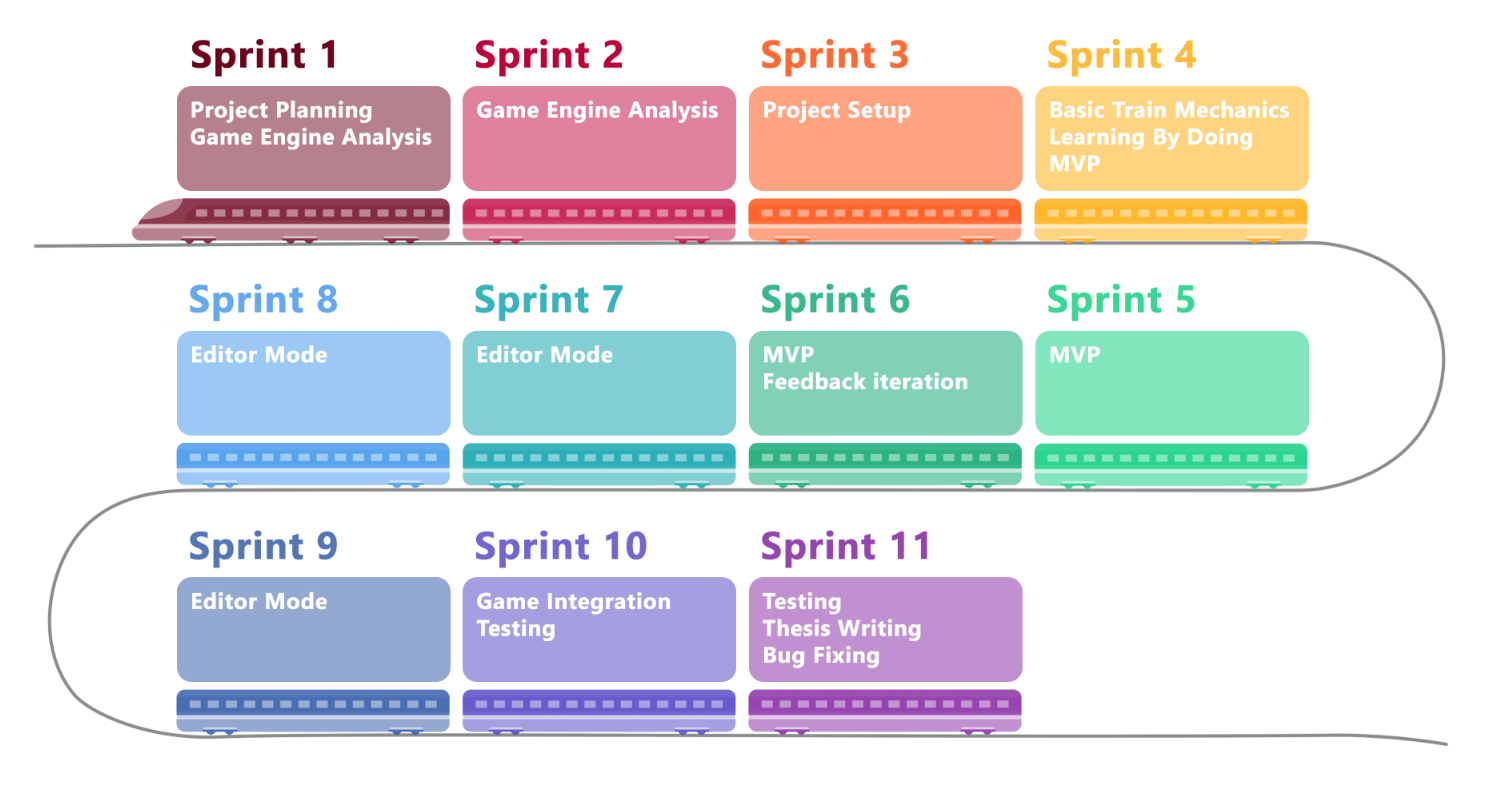
\includegraphics[width=14cm]{figures/ExampleSprintOverview.png}
    %\vspace{-12pt}
    \caption{Overview of all Sprints}
    \label{sprint_overview_img}
\end{figure} 

The scrum meetings are written with three different sections. A section about the Goals we have for the sprint. A section we write when the sprint is completed, which covers the result of the sprint. And a retrospective section where we will discuss and reflect on the result of the sprint with the goals in mind. \\

\textbf{Statuses} \\
The issues in a sprint can be set to one of five different statuses. The statuses are respectively: \textbf{Wishlist} - The issues that is taken out of the project scope and in to a list of functionality that we can decide to include if we have time later in the project. \textbf{To Do} - This are the section for issues that are waiting to be developed. \textbf{In Progress} - The issues that are currently being developed. \textbf{Done} - The issues that has been completed in the sprint.
\\


\begin{large}
\textbf{Sprint 4} \\
\end{large}
\textbf{Date:} 14.02.2022 \\ 
\textbf{Present:} Endre, Henrik, John Ole and Thomas \\
\textbf{Period:} 14.02 - 21.02 \\ 
\\
\begin{table}[H]
    \centering
    \begin{tblr}{
      colspec={|X[0.20, c]|X[0.20, c]|X[0.25, c]|X[0.35, c]|}, hlines,
      column{1} = {gray9},
      column{2} = {blue9},
      column{3} = {yellow9},
      column{4} = {green9},
    }
    \SetCell{bg=gray4}  
    & \textbf{To do} 
    & \textbf{In progress}  
    & \textbf{Done} \\
    Issues 
    & \SetCell[c=1]{l}  Railway integration (7) \newline \newline Curvature warnings (7)
    & \SetCell[c=1]{l} Environment: \newline - Modeling (7) \newline  - Texturing (3)  \newline - Foliage (3) \newline \newline Basic statuses (3)
    & \SetCell[c=1]{l} Input Handling (7) \newline \newline Calculate acceleration (3) \newline \newline Move along Path (7) \newline \newline Signals: \newline \newline Add Models (3) \newline \newline Railway: \newline \newline - Procedural mesh (7) \newline \newline Spline Formation (14) \\
        Estimates & 14 & 16 & 41 
    \end{tblr}
\end{table} 
\bigskip \bigskip

\textbf{Sprint Goal:} \\
\begin{itemize}
    \item Finish the basic train mechanics
    \item Finish the first MVP level environment
    \item Finish the Basic spline railway
\end{itemize}

\textbf{Sprint result:} \\
We set out the sprint with very high expectations because of the delays we have had in previous sprints. All the basic train mechanics and the railway got finished as well as some of the environment and signals. 

\textbf{Retrospective:} \\
One of the group members lost some work days because of sickness. We underestimated the time it takes too model, texture and set up foliage for the environment. Thees tasks should each have been estimated as a 3 and is together with the sickness the reason we did not finish all tasks this sprint. We decided to re-estimate the tasks left from the previous sprint and therefore all of the environment tasks will be set as 3 and the basic statuses will also be set on 3. Basic statuses involves more complex functionality than first expected. 

We had a plan to use the estimations of 1 = 3 hours, 2 = 7 hours and 3 = 14 hours, but we decided to change this. The reason we want to change the estimation is because we feel that it is not accurate enough and we should not restrict our estimation process to only three categories. We therefore decided that further estimations should be done by hours alone and not by a predetermined scale.


\begin{large}
    \textbf{Sprint 5} \\
\end{large}
\textbf{Date:} 21.02.2022 \\ 
\textbf{Present:} Endre, Henrik, John Ole and Thomas \\
\textbf{Period:} 21.02 - 28.02 \\ 
\newline
\begin{table}[H]
    \centering
    \begin{tblr}{
      colspec={|X[0.15, c]|X[0.21, c]|X[0.21, c]|X[0.21, c]|X[0.21, c]|}, hlines,
      column{1} = {gray9},
      column{2} = {purple9},
      column{3} = {blue9},
      column{4} = {blue9},
      column{5} = {green9},
    }
    \SetCell{bg=gray4}  &
    \textbf{Wishlist} &
    \textbf{To do} &
    \textbf{In progress} &
    \textbf{Done} \\
        Issues 
        & \SetCell[c=1]{l} Curvature Warnings (10)
        & \SetCell[c=1]{l} Speed Limit Indicator (10) \newline \newline Signals: \newline  - Railway Integration (4)
        & \SetCell[c=1]{l} Basic Statuses (20) \newline \newline Environment:
        - Modeling (14) \newline - Texturing(12) \newline - Foliage(12) \newline \newline Add Speedometer(8)
        & \SetCell[c=1]{l} Drone Mode (7) \newline \newline Spline Terrain Adaptation (10) \newline \newline Main Menu (7) \newline \newline Popup Message (3) \newline \newline In Game Menu (4) \newline \newline Options Menu (10)\\
        Estimates & 10 & 14 & 66 & 41
    \end{tblr}
\end{table}
\bigskip \bigskip

\textbf{Sprint Goal:} \\
\begin{itemize}
    \item Finish Main Menu in game menu and pop-up messages
    \item Finish basic statuses
    \item Finish The environment creation
\end{itemize}

\textbf{Sprint result:} \\
All the initial UI got finished in blueprints. The environment creation is nearly finished. The basic statuses task was increasing in size because...

\textbf{Retrospective:} \\
The sprint was set to contain 121 work hours, this is all the time we as a group has for a full week since every group member should have 30 hours of work each week.We only finished work hours of about 41 estimated hours. And we estimate that half of the in progress tasks are finished. This puts our completed work to 74 hours. We have underestimated both the time and complexity of several tasks. We have to use this knowledge on further estimations meaning we have to estimate issues with a larger margin of error


\begin{large}
    \textbf{Sprint 6} \\
\end{large}
\textbf{Date:} 28.02.2022 \\ 
\textbf{Present:} Endre, Henrik, John Ole and Thomas \\
\textbf{Period:} 28.02 - 07.03 \\ 
\newline
\begin{table}[H]
    \centering
    \begin{tblr}{
      colspec={|X[0.15, c]|X[0.20, c]|X[0.20, c]|X[0.45, c]|}, hlines,
      column{1} = {gray9},
      column{2} = {purple9},
      column{3} = {blue9},
      column{4} = {green9},
    }
    \SetCell{bg=gray4}  &
    \textbf{Wishlist} &
    \textbf{In progress} &
    \textbf{Done} \\
        Issues 
        & \SetCell[c=1]{l} Speed Limit Indicator (10) \newline \newline
        & \SetCell[c=1]{l} Basic Statuses (5)
        & \SetCell[c=1]{l} Environment Creation: \newline - Moddeling (10) \newline - Texturing (10) \newline - Folaige (10) \newline \newline Add speedometer (4) \newline \newline Requirement specification (20) \newline \newline Status report 1 (10) \newline \newline Signals: \newline - Railway integration (4) \newline \newline Gravel Mesh Under Spline (10) \newline \newline Bug: \newline - Spline hovering above ground (15) \\
        Estimates & 10 & 5 & 93 
    \end{tblr}
\end{table}
\bigskip \bigskip

\textbf{Sprint Goal:} \\
\begin{itemize}
    \item Finish first draft of requirement specification and status report 1.
    \item Finish the MVP scenario
\end{itemize}

\textbf{Sprint result:} \\
The MVP got finished and put together. We had some issues with the environment creation and it's time consumption, but the estimations we made for three environment creation tasks was more accurate than our previous estimations. All the necessary functionality was there to display the MVP to the client except the basic statuses which we only controlled by a timer instead of an controller. The basic statuses only misses a few hours of work and is therefore almost finished.

\textbf{Retrospective:} \\
The sprint goals was achieved, but the basic statuses was only implemented to work with the MVP scenario and not finished to he extent we want in the final product. We want the signals to be controlled by a controller and be able to trigger events. New issues for this will come in the next sprint. We finished 93 work hours in the sprint and we feel that our estimations on the different tasks are beginning to get better and more accurate to how we progress in the sprints. We decided after this retrospective meeting to increase the size of the sprints from one to two weeks for the upcoming sprints. We are now going to work on two milestones simultaneously and feel that a two week sprint will give us time to produce more and that the development will be more efficient. 



\begin{large}
    \textbf{Sprint 7} \\
\end{large}
\textbf{Date:} 07.03.2022 \\ 
\textbf{Present:} Endre, Henrik, John Ole and Thomas \\
\textbf{Period:} 07.03 - 21.03 \\ 
\newline
\begin{table}[H]
    \centering
    \begin{tblr}{
      colspec={|X[0.15, c]|X[0.21, c]|X[0.21, c]|X[0.21, c]|X[0.22, c]|}, hlines,
      column{1} = {gray9},
      column{2} = {purple9},
      column{3} = {blue9},
      column{4} = {blue9},
      column{5} = {green9},
    }
    \SetCell{bg=gray4}  &
    \textbf{Wishlist} &
    \textbf{To do} &
    \textbf{In Progress} &
    \textbf{Done} \\
        Issues 
        & \SetCell[c=1]{l} Editor mode: \newline - Generate flat terrain (14) \newline - Manipulate terrain (20) \newline - Dynamic buttons (10)
        & \SetCell[c=1]{l} Place and edit railway (28) \newline \newline Load scenario from file (14) \newline \newline Save scenario to file (14) Static Buttons on screen (7)
        & \SetCell[c=1]{l} Main Goal: \newline - Signal Controller (21) \newline - Emergency Breaks (7) \newline - Stop Scenario (21) \newline \newline In game content browser (25) \newline \newline Save Object to File (20) \newline \newline Load Object From File (20)
        & \SetCell[c=1]{l} Main Menu (14) \newline \newline Basic Statuses (7) \newline \newline Second iteration Requirement Specification (21)  \newline \newline Place 3D Models (12) \newline \newline Manipulate 3D Models (25)  \\
        Estimates & 44 & 63 & 114 & 79
    \end{tblr}
\end{table}
\bigskip \bigskip

\textbf{Sprint Goal:} \\
\begin{itemize}
    \item Finish first draft of requirement specification and status report 1.
    \item Finish the MVP scenario
\end{itemize}

\textbf{Sprint result:} \\
The MVP got finished and put together. We had some issues with the environment creation and it's time consumption, but the estimations we made for three environment creation tasks was more accurate than our previous estimations. All the necessary functionality was there to display the MVP to the client except the basic statuses which we only controlled by a timer instead of an controller. The basic statuses only misses a few hours of work and is therefore almost finished.

\textbf{Retrospective:} \\
The sprint goals was achieved, but the basic statuses was only implemented to work with the MVP scenario and not finished to he extent we want in the final product. We want the signals to be controlled by a controller and be able to trigger events. New issues for this will come in the next sprint. We finished 93 work hours in the sprint and we feel that our estimations on the different tasks are beginning to get better and more accurate to how we progress in the sprints.


\begin{large}
    \textbf{Sprint 8} \\
\end{large}
\textbf{Date:} 22.03.2022 \\ 
\textbf{Present:} Endre, Henrik, John Ole and Thomas \\
\textbf{Period:} 22.03 - 04.04 \\ 
\newline
\begin{table}[H]
    \centering
    \begin{tblr}{
      colspec={|X[0.15, c]|X[0.21, c]|X[0.21, c]|X[0.21, c]|X[0.22, c]|}, hlines,
      column{1} = {gray9},
      column{2} = {purple9},
      column{3} = {blue9},
      column{4} = {blue9},
      column{5} = {green9},
    }
    \SetCell{bg=gray4}  &
    \textbf{Wishlist} &
    \textbf{To do} &
    \textbf{In Progress} &
    \textbf{Done} \\
        Issues 
        & \SetCell[c=1]{l} Editor mode: \newline - Save Scenario to File (14) \newline - Load Scenario from File (20) 
        & \SetCell[c=1]{l}Static Buttons on Screen (7) \newline \newline Place and Edit railways (28)
        & \SetCell[c=1]{l} Save Object to File (20) \newline \newline Load Object From File (20) \newline \newline Log In: \newline - Add User Types (10) \newline - Restrict functionalities (10)
        & \SetCell[c=1]{l} Main Goal: \newline - Signal Controller (21) \newline - Emergency Breaks (7) \newline - Stop Scenario (21) \newline \newline In game content browser (15)  \newline \newline Third Iteration Requirement Spesification (10)\\
        Estimates & 34 & 35 & 60 & 74
    \end{tblr}
\end{table}
\bigskip \bigskip

\textbf{Sprint Goal:} \\
\begin{itemize}
    \item Finish the editor mode, meaning the content browser and all the tools for saving, placing and the UI.
    \item Finish the third iteration of the requirement specification.
    \item Finish the Main Goal which is a working scenario with a controller for the signals.
\end{itemize}

\textbf{Sprint result:} \\
We finished the third iteration of the requirement document and the main goal. The editor mode is about halfway done. 

\textbf{Retrospective:} \\
The estimations we made was not very accurate to the workload. the content browser for example has been challenging to get working. This is because it introduced many problems that we did not account for when estimating. This issue which we thought initially would take approximately 4 days to complete has now been a work in progress for about two weeks. Because of the troubles we have had we will use the next sprint (which includes the easter) to continue working towards finishing up the editor mode.

\begin{large}
    \textbf{Sprint 9} \\
\end{large}
\textbf{Date:} 04.03.2022 \\ 
\textbf{Present:} Endre, Henrik, John Ole and Thomas \\
\textbf{Period:} 04.04 - 13.04 \\ 
\newline

\begin{table}[H]
    \centering
    \begin{tblr}{
      colspec={|X[0.15, c]|X[0.42, c]|X[0.43, c]|}, hlines,
      column{1} = {gray9},
      column{2} = {blue9},
      column{3} = {green9},
    }
    \SetCell{bg=gray4}  &
    \textbf{In Progress} &
    \textbf{Done} \\
        Issues 
        & Place and Edit railways (28)
        & \SetCell[c=1]{l} Save Object to File (5) \newline \newline Load Object From File (5) \newline \newline Log In: \newline - Add User Types (7) \newline - Restrict functionalities (7) \newline \newline Static buttons on screen (25) \newline \newline Fourth iteration Requirement Specification (10) \newline \newline Bachelor Thesis draft (20) \\
        Estimates & 28 & 79
    \end{tblr}
\end{table}
\bigskip \bigskip

\textbf{Sprint Goal:} \\
\begin{itemize}
    \item Finish the editor mode, meaning the content browser and all the tools for saving, placing and the UI.
    \item Finish the fourth iteration of the requirement specification and deliver a draft of the thesis.
\end{itemize}

\textbf{Sprint result:} \\
We finished both the requirement specification and the requirement specification. The place and edit railway issue was started but there was some issues with the relevancy and meaning of including it in the project. 

\textbf{Retrospective:} \\
On our meeting with the supervisor he brought up that it may be necessary to cut out the railway editing tool. Our discussion on the subject. We figured that because of the problems we have had with it and the fact that the functionality we can produce would not be better than using the original spline tool in the UE4 editor we decided that Thomas will work on the issue for one more day to see find out if the issue is worth resolving or if it's smarter to cut out the functionality and focus on other parts of the project.
Update, the place and edit railways issue will be excluded from the backlog because we want to focus on other parts of the assignment.

%%%%%%%%%%%%%%%%%%%%%%%%%%%%%%%%%%%% SCRUM %%%%%%%%%%%%%%%%%%%%%%%%%%%%%%%%%%%%%%%%%%



\subsection{Deviation from original plan}
\bigskip
\begin{figure}[H]
    \centering
    \vspace{12pt}
    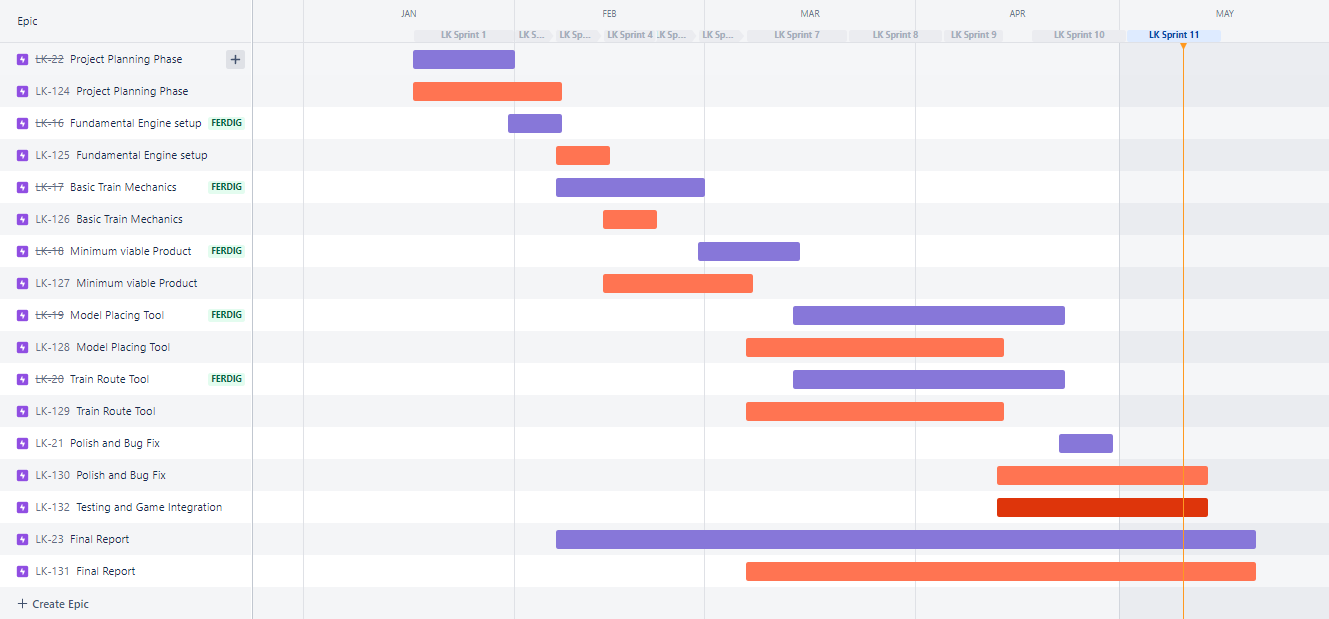
\includegraphics[width=12cm]{figures/Jira comparisoncroped.png}
    \caption{Comparison of }
    \label{Epic_comparison_img}
\end{figure} 
\bigskip \bigskip




- stopped doing daily meetings, felt it was not needed - most meetings were spent repeating already known info 

- after the main goal mvp was done we switched from 1 week to 2 week sprints, as we felt the tasks ahead required more time to develop and progress. using 2 week sprints allows the group to take a day off after a sprint to work on other stuff unrelated to the issues in the sprint if they want. When having 1 week sprints the time spent developing vs time spent planning is (not enough we feel). 

